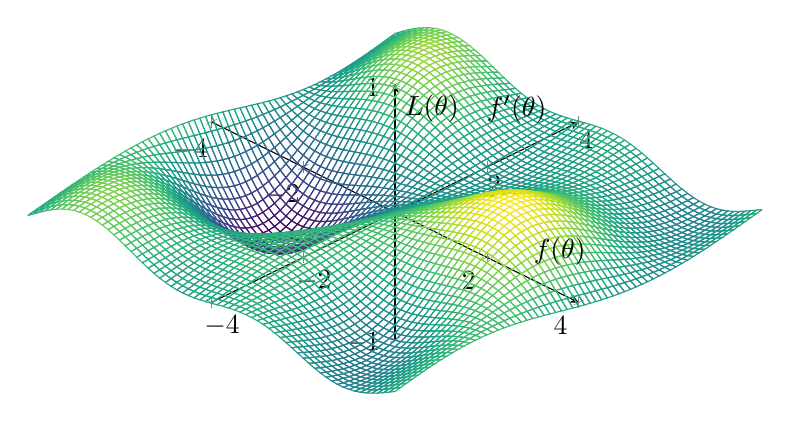
\begin{tikzpicture}
\begin{axis}[
    width=0.9\textwidth,
    view={45}{45},
    axis lines=center,
    xlabel={$f(\theta)$},
    ylabel={$f'(\theta)$},
    zlabel={$L(\theta)$},
    domain=-4:4,
    y domain=-4:4,
    zmin=-1, zmax=1,
    samples=65,
    samples y=65,
    colormap/viridis,
    % colorbar,
]
\addplot3[
    surf,
    mesh,
    shader=interp,
    point meta=rawz,
]
{
0.5*sin(deg(0.8*x))*cos(deg(0.8*y))
* exp(-0.1*(x + y^2))
- 0.1*sin(deg(1.6*x + 0.8*y))
};

\end{axis}
\end{tikzpicture}